\documentclass[aspectratio=169]{beamer}

\usetheme{Madrid}
\usecolortheme{default}
\usepackage{booktabs}
\usepackage{amsmath}
\usepackage{graphicx}
\usepackage{tikz}
\usetikzlibrary{arrows.meta, positioning, shapes.geometric, calc}

\definecolor{highformal}{RGB}{44,123,182}
\definecolor{semiformal}{RGB}{253,174,97}
\definecolor{lowformal}{RGB}{215,48,39}
\definecolor{nwgreen}{RGB}{76,153,0}

\title{From OWL to EER to Natural Language}
\subtitle{How Representation Formality Shapes LLM Reasoning\\over Conceptual Models}
\author{Wolfgang Maa\ss \and Veda C.\ Storey \and Stephen W.\ Liddle}
\institute{DFKI \and Georgia State University \and Brigham Young University}
\date{ER 2026}

\begin{document}

% ══════════════════════════════════════════════════════════════
\begin{frame}
\titlepage
\end{frame}

% ══════════════════════════════════════════════════════════════
\begin{frame}{Motivation}

\begin{columns}[T]
\begin{column}{0.55\textwidth}
\textbf{Conceptual models vary in formalization:}
\begin{itemize}
    \item \textbf{Formal:} OWL ontology --- precise syntax, model-theoretic semantics, automated reasoning
    \item \textbf{Semi-formal:} EER diagram --- constrains interpretation without full formality
    \item \textbf{Informal:} NL requirements --- open syntax and semantics
\end{itemize}

\vspace{0.5em}
\textbf{Research question:}\\
Does the formalization level of a CM representation predict how well an LLM can reason over it?

\vspace{0.5em}
\textit{Mylopoulos (1992), Wand \& Weber (1990)}
\end{column}

\begin{column}{0.42\textwidth}
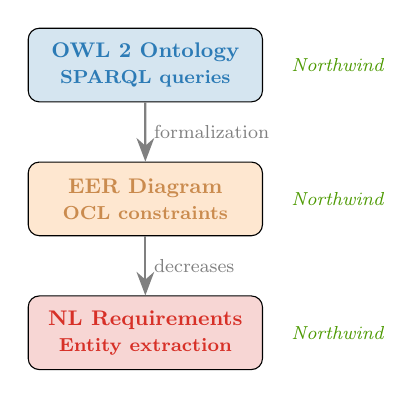
\begin{tikzpicture}[
    level/.style={draw, rounded corners, minimum width=3.5cm, minimum height=1.1cm, align=center, font=\small\bfseries},
    arr/.style={-{Stealth[length=3mm]}, thick, gray},
    scale=0.85, transform shape
]
\node[level, fill=highformal!20, text=highformal] (high) at (0,4) {OWL 2 Ontology\\{\footnotesize SPARQL queries}};
\node[level, fill=semiformal!30, text=semiformal!80!black] (semi) at (0,2) {EER Diagram\\{\footnotesize OCL constraints}};
\node[level, fill=lowformal!20, text=lowformal] (low) at (0,0) {NL Requirements\\{\footnotesize Entity extraction}};

\draw[arr] (high) -- node[right, font=\footnotesize, text=gray] {formalization} (semi);
\draw[arr] (semi) -- node[right, font=\footnotesize, text=gray] {decreases} (low);

\node[font=\footnotesize\itshape, text=nwgreen, right=0.3cm] at (high.east) {Northwind};
\node[font=\footnotesize\itshape, text=nwgreen, right=0.3cm] at (semi.east) {Northwind};
\node[font=\footnotesize\itshape, text=nwgreen, right=0.3cm] at (low.east) {Northwind};
\end{tikzpicture}
\end{column}
\end{columns}

\end{frame}

% ══════════════════════════════════════════════════════════════
\begin{frame}{Research Hypotheses}

\begin{description}[H3:]
    \item[H1:] \textbf{Quality gradient.} LLM output quality decreases monotonically as task formalization decreases.
    \vspace{0.5em}
    \item[H2:] \textbf{Variance gradient.} Output variance across repeated runs increases as formalization decreases.\\
    {\small\color{gray} (Prior work: refuted --- formal tasks produce \emph{higher} variance due to bimodal hit-or-miss distributions.)}
    \vspace{0.5em}
    \item[H3:] \textbf{Length--quality mediation.} Response length positively mediates recall-based quality scores across formalization levels.
\end{description}

\vspace{1em}
\textbf{Key innovation:} Same domain (Northwind) across all three levels --- domain confound eliminated.

\end{frame}

% ══════════════════════════════════════════════════════════════
\begin{frame}{Theoretical Grounding}

\begin{columns}[T]
\begin{column}{0.48\textwidth}
\textbf{SEQUAL Framework} {\small(Krogstie et al.\ 1995)}\\[0.3em]
$F(T)$ maps onto SEQUAL quality dimensions:
\vspace{0.3em}

\begin{tabular}{@{}ll@{}}
\toprule
$F(T)$ & SEQUAL \\
\midrule
$S(T)$ syntactic density & Syntactic quality \\
$D(T)$ decidability & Pragmatic quality \\
$C(T)$ cardinality & Semantic quality$^{-1}$ \\
\bottomrule
\end{tabular}

\vspace{0.8em}
$F(T) = \tfrac{1}{3}(\hat{C}(T) + S(T) + D(T))$

\vspace{0.3em}
{\small $F \approx 0.89$ (OWL), $0.50$ (EER), $0.17$ (NL)}
\end{column}

\begin{column}{0.48\textwidth}
\textbf{Moody's Physics of Notations} {\small(2009)}\\[0.3em]
Three principles extend to LLMs:
\vspace{0.3em}
\begin{itemize}
    \item \textbf{Semiotic clarity:} OWL constructs have unambiguous semantics $\rightarrow$ consistent training signal
    \item \textbf{Semantic transparency:} OWL reduces per-token disambiguation burden
    \item \textbf{Complexity management:} Modular class hierarchies reduce context-window load
\end{itemize}

\vspace{0.5em}
{\small\color{gray} Visual principles (perceptual discriminability, etc.)\ explicitly excluded.}
\end{column}
\end{columns}

\end{frame}

% ══════════════════════════════════════════════════════════════
\begin{frame}{Experimental Design --- Single Domain, Three Levels}

\begin{table}
\centering
\small
\begin{tabular}{p{1.8cm}p{3.5cm}p{3.5cm}p{3.2cm}}
\toprule
& \textbf{\color{highformal}High-Formal} & \textbf{\color{semiformal!80!black}Semi-Formal} & \textbf{\color{lowformal}Low-Formal} \\
\midrule
Representation & OWL 2 DL ontology (Turtle) & EER diagram (structured prose) + NL annotations & NL requirements document \\[0.5em]
Domain & \multicolumn{3}{c}{\textbf{Northwind} (food distribution: customers, orders, products, suppliers, employees)} \\[0.5em]
Tasks & 100 SPARQL competency questions & 59 tasks across 11 EER categories & 31 tasks across 9 requirements categories \\[0.5em]
Evaluation & Reasoner-verified (HermiT + Jena) & OCL parse/typecheck + expert rubric & Entity coverage vs.\ gold EER + expert rubric \\[0.5em]
$F(T)$ & $\approx 0.89$ & $\approx 0.50$ & $\approx 0.17$ \\
\bottomrule
\end{tabular}
\end{table}

\vspace{0.3em}
\centering
{\small 190 tasks $\times$ 2 models $\times$ $K\!=\!5$ runs = \textbf{1,900 total records}}

\end{frame}

% ══════════════════════════════════════════════════════════════
\begin{frame}{High-Formal Task: Generate SPARQL from an OWL Ontology}

{\small
\textbf{Model receives:} Northwind OWL 2 ontology (Turtle, 11 classes, ${\sim}100$ axioms) + NL question \quad
\textbf{Must produce:} SPARQL query \quad
\textbf{Verified by:} Execution in Apache Jena}

\vspace{0.3em}
\begin{columns}[T]
\begin{column}{0.48\textwidth}
\colorbox{highformal!8}{\parbox{0.95\linewidth}{\footnotesize
\textbf{Input (question):}\\[0.2em]
\textit{``List customers who have ordered a discontinued product.''}\\[0.4em]
\textbf{Input (ontology excerpt):}\\[0.2em]
{\scriptsize\ttfamily
nw:Order rdfs:subClassOf [\\
~~owl:onProperty nw:hasOrderLine ;\\
~~owl:minCardinality 1 ] .\\
nw:placedBy rdfs:domain nw:Order ;\\
~~rdfs:range nw:Customer .\\
nw:discontinued rdfs:domain nw:Product ;\\
~~rdfs:range xsd:boolean .
}}}
\end{column}

\begin{column}{0.49\textwidth}
\colorbox{highformal!8}{\parbox{0.95\linewidth}{\footnotesize
\textbf{Expected output (gold SPARQL):}\\[0.2em]
{\scriptsize\ttfamily
PREFIX nw: <\ldots/northwind\#>\\
SELECT DISTINCT ?cname ?pname\\
WHERE \{\\
~~?o nw:placedBy ?c .\\
~~?c nw:companyName ?cname .\\
~~?o nw:hasOrderLine ?line .\\
~~?line nw:includesProduct ?p .\\
~~?p nw:productName ?pname .\\
~~?p nw:discontinued "true"\^{}\^{}xsd:boolean .\\
\}
}\\[0.3em]
\textbf{Verification:} Jena returns ``Com\'{e}rcio Mineiro, Guaran\'{a} Fant\'{a}stica''
}}
\end{column}
\end{columns}

\vspace{0.4em}
{\footnotesize 100 tasks: simple retrieval (15), property traversal (20), multi-hop join (20), aggregation (15), constraint reasoning (15), negation (15)}

\end{frame}

% ══════════════════════════════════════════════════════════════
\begin{frame}{Semi-Formal Task: Reason over an EER Diagram with NL Annotations}

{\small
\textbf{Model receives:} Northwind EER diagram (structured prose with NL annotations) + question \quad
\textbf{Must produce:} OCL constraint or reasoned answer \quad
\textbf{Verified by:} OCL parse/typecheck + expert rubric}

\vspace{0.3em}
\begin{columns}[T]
\begin{column}{0.47\textwidth}
\colorbox{semiformal!10}{\parbox{0.95\linewidth}{\footnotesize
\textbf{Input (EER diagram excerpt):}\\[0.2em]
{\scriptsize\ttfamily
WEAK ENTITY OrderLine \{\\
~~Partial key: lineNumber\\
~~Owner: Order (via Contains)\\
~~\textbf{Note: The quantity ordered}\\
~~\textbf{must be a positive integer.}\\
\}}\\[0.4em]
\textbf{Task (OCL synthesis):}\\[0.2em]
\textit{``Formalize the annotation on OrderLine as an OCL invariant.''}
}}

\vspace{0.2em}
\colorbox{semiformal!10}{\parbox{0.95\linewidth}{\footnotesize
\textbf{Expected output:}\\[0.2em]
{\scriptsize\ttfamily
context OrderLine\\
inv positiveQuantity: self.quantity > 0
}}}
\end{column}

\begin{column}{0.50\textwidth}
\colorbox{semiformal!10}{\parbox{0.95\linewidth}{\footnotesize
\textbf{Input (same diagram, different task):}\\[0.2em]
{\scriptsize\ttfamily
RELATIONSHIP Contains \{\\
~~Order (total, 1), OrderLine (total, N)\\
\}}\\[0.4em]
\textbf{Task (participation inference):}\\[0.2em]
\textit{``What does total participation of OrderLine in Contains imply for DELETE on Order?''}
}}

\vspace{0.2em}
\colorbox{semiformal!10}{\parbox{0.95\linewidth}{\footnotesize
\textbf{Expected output:}\\[0.2em]
\textit{``Deleting an Order must cascade-delete all its OrderLines --- an OrderLine cannot exist without its owning Order. Enforce via CASCADE or RESTRICT.''}
}}

\vspace{0.3em}
{\footnotesize 59 tasks across 11 categories (OCL synthesis, weak entity, cardinality violation, participation inference, \ldots)}
\end{column}
\end{columns}

\end{frame}

% ══════════════════════════════════════════════════════════════
\begin{frame}{Low-Formal Task: Extract Structure from NL Requirements}

{\small
\textbf{Model receives:} NL requirements document (prose only --- no schema, no diagram) + CM question \quad
\textbf{Must produce:} Entities, relationships, constraints, or ambiguity analysis \quad
\textbf{Verified by:} Coverage vs.\ gold EER + expert rubric}

\vspace{0.3em}
\begin{columns}[T]
\begin{column}{0.47\textwidth}
\colorbox{lowformal!8}{\parbox{0.95\linewidth}{\footnotesize
\textbf{Input (requirements excerpt):}\\[0.2em]
\textit{``Each customer may place multiple orders over time, or none at all. Every order must be associated with exactly one customer. Each order is made up of one or more order lines\ldots''}\\[0.4em]
\textbf{Task (entity identification):}\\[0.2em]
\textit{``Identify all candidate entities for a data model of this system.''}
}}

\vspace{0.2em}
\colorbox{lowformal!8}{\parbox{0.95\linewidth}{\footnotesize
\textbf{Expected output:}\\[0.2em]
\textit{Customer, Order, OrderLine, Product}\\[0.1em]
\textbf{Coverage:} 4/5 gold entities (Employee typically missed)
}}
\end{column}

\begin{column}{0.50\textwidth}
\colorbox{lowformal!8}{\parbox{0.95\linewidth}{\footnotesize
\textbf{Input (same document, different task):}\\[0.2em]
\textit{``\ldots Products can be marked as discontinued; once discontinued, a product \textbf{should} not appear on any new orders\ldots''}\\[0.4em]
\textbf{Task (ambiguity flagging):}\\[0.2em]
\textit{``Flag the modeling implications of the word `should.'\,''}
}}

\vspace{0.2em}
\colorbox{lowformal!8}{\parbox{0.95\linewidth}{\footnotesize
\textbf{Expected output:}\\[0.2em]
\textit{``Should'' is ambiguous --- hard constraint (reject INSERT) vs.\ soft guideline (warn + allow). Modeling consequences: integrity constraint vs.\ application-layer check with override.}
}}

\vspace{0.3em}
{\footnotesize 31 tasks across 9 categories (entity ID, relationship ID, cardinality inference, ambiguity flagging, constraint elicitation, \ldots)}
\end{column}
\end{columns}

\end{frame}

% ══════════════════════════════════════════════════════════════
\begin{frame}{Evaluation Design}

\begin{columns}[T]
\begin{column}{0.48\textwidth}
\textbf{Unified 0--3 expert rubric}\\[0.3em]
{\small
\begin{tabular}{@{}cp{5.5cm}@{}}
\toprule
Score & Criteria \\
\midrule
3 & Correct and complete (execution-verified / structurally + semantically correct / full coverage) \\
2 & Substantially correct, minor gaps \\
1 & Partial --- some relevant content, major errors \\
0 & Incorrect, irrelevant, or hallucinated \\
\bottomrule
\end{tabular}
}

\vspace{0.5em}
{\small Two independent annotators\\Cohen's $\kappa \geq 0.70$ per level}
\end{column}

\begin{column}{0.48\textwidth}
\textbf{Level-specific automated metrics:}\\[0.3em]
{\small
\begin{tabular}{@{}ll@{}}
\toprule
Level & Automated check \\
\midrule
High & SPARQL execution (Jena) \\
Semi & OCL parse + typecheck \\
Low & Entity/rel.\ coverage vs.\ EER \\
\bottomrule
\end{tabular}
}

\vspace{0.8em}
\textbf{Statistical pipeline:}
\begin{itemize}\small
    \item Kruskal-Wallis (H1 omnibus)
    \item Mann-Whitney U + Bonferroni
    \item Levene's test (H2 variance)
    \item Rank-biserial effect size
\end{itemize}
\end{column}
\end{columns}

\end{frame}

% ══════════════════════════════════════════════════════════════
\begin{frame}{Models and Infrastructure}

\begin{columns}[T]
\begin{column}{0.48\textwidth}
\textbf{Models:}
\begin{itemize}
    \item \textbf{Mistral-7B-Instruct-v0.3}\\7.24B params, sliding-window attention
    \item \textbf{Llama-3.1-8B-Instruct}\\8.03B params, 128K context, RoPE
\end{itemize}

\vspace{0.5em}
Both run locally on NVIDIA A100 40GB\\(HPC cluster, FP16, $T\!=\!0.7$)

\vspace{0.5em}
Each task executed $K\!=\!5$ times\\for consistency analysis
\end{column}

\begin{column}{0.48\textwidth}
\textbf{Toolchain:}
\begin{itemize}
    \item \textbf{HermiT 1.4} --- ontology consistency verification
    \item \textbf{Apache Jena} --- SPARQL execution against populated ABox
    \item \textbf{Dresden OCL} --- OCL parse and typecheck against Ecore metamodel
    \item \textbf{HuggingFace Transformers} --- model inference
    \item \textbf{Neuron activation tracking} --- MLP layer instrumentation
\end{itemize}
\end{column}
\end{columns}

\end{frame}

% ══════════════════════════════════════════════════════════════
\begin{frame}{Pilot Results: High-Formal (SPARQL, 5 tasks $\times$ $K\!=\!5$)}

\begin{columns}[T]
\begin{column}{0.48\textwidth}
\textbf{SPARQL execution rate:}\\[0.3em]
{\small
\begin{tabular}{@{}lcc@{}}
\toprule
Task & Mistral & Llama \\
\midrule
HF-1 (simple) & 2/5 & 0/5 \\
HF-2 (simple) & 3/5 & 0/5 \\
HF-3 (medium) & 3/5 & 0/5 \\
HF-4 (medium) & 0/5 & 0/5 \\
HF-5 (hard) & 3/5 & 0/5 \\
\midrule
\textbf{Total} & \textbf{11/25 (44\%)} & \textbf{0/25 (0\%)} \\
\bottomrule
\end{tabular}
}

\vspace{0.5em}
{\small Mistral improved from 20\% $\rightarrow$ 44\% with prompt engineering and extraction fixes.}
\end{column}

\begin{column}{0.48\textwidth}
\textbf{Llama failure mode:}\\[0.3em]
{\small Missing spaces after \texttt{?} in variable names (\texttt{SELECT?name} instead of \texttt{SELECT~?name}) causes Jena parse failures. Query \emph{structure} is often correct.}

\vspace{0.8em}
\textbf{Mistral failure mode:}\\[0.3em]
{\small HF-4 (aggregation + HAVING) fails consistently --- both models struggle with GROUP BY / HAVING in SPARQL.}

\vspace{0.8em}
\textbf{Key insight:}\\
{\small Models understand the ontology structure (correct property traversal) but produce syntactically fragile SPARQL. Post-processing can recover ${\sim}68\%$ from Mistral's raw outputs.}
\end{column}
\end{columns}

\end{frame}

% ══════════════════════════════════════════════════════════════
\begin{frame}{Pilot Results: Semi-Formal and Low-Formal}

\begin{columns}[T]
\begin{column}{0.48\textwidth}
\textbf{Semi-Formal --- OCL go/no-go:}\\[0.3em]
{\small
\begin{tabular}{@{}lcc@{}}
\toprule
& Mistral & Llama \\
\midrule
OCL presence & 60\% & 80\% \\
OCL parse & 60\% & 80\% \\
OCL typecheck & 30\% & 60\% \\
\bottomrule
\end{tabular}
}

\vspace{0.3em}
$\rightarrow$ Both $\geq 25\%$ threshold: \textbf{proceed with OCL}

\vspace{0.5em}
{\small Non-OCL tasks (weak entity, participation constraints, cardinality violations): both models answer correctly with diagram references.}

\vspace{0.5em}
\textbf{Llama outperforms on OCL:}\\
{\small 80\% presence vs.\ Mistral's 60\%.\\Higher typecheck rate (60\% vs.\ 30\%).}
\end{column}

\begin{column}{0.48\textwidth}
\textbf{Low-Formal --- entity coverage:}\\[0.3em]
{\small
\begin{tabular}{@{}lcc@{}}
\toprule
Task & Mistral & Llama \\
\midrule
LF-1 (entity ID) & 84\% & 84\% \\
LF-2 (relationship ID) & 80\% & 80\% \\
LF-3 (cardinality) & 40\% & 40\% \\
LF-4 (ambiguity) & 60\% & 76\% \\
LF-5 (constraint) & 80\% & 80\% \\
\midrule
\textbf{Average} & \textbf{69\%} & \textbf{72\%} \\
\bottomrule
\end{tabular}
}

\vspace{0.5em}
\textbf{Response length ordering:}\\[0.2em]
{\small
\begin{tabular}{@{}lccc@{}}
& High & Semi & Low \\
\midrule
Mistral & 412 & 439 & 1{,}289 \\
Llama & 1{,}725 & 4{,}378 & 4{,}421 \\
\end{tabular}
}

\vspace{0.2em}
{\small Mistral: high $<$ semi $<$ low \checkmark\\Llama: high $<$ semi $\approx$ low}
\end{column}
\end{columns}

\end{frame}

% ══════════════════════════════════════════════════════════════
\begin{frame}{Pilot Results: Stage 4 Decisions and Emerging Patterns}

\begin{columns}[T]
\begin{column}{0.50\textwidth}
\textbf{Go/no-go decisions:}\\[0.5em]
{\small
\begin{tabular}{@{}lll@{}}
\toprule
Decision & Result & Status \\
\midrule
D1: SPARQL & Mistral 44\% & \textbf{Proceed} \\
D2: OCL & 60--80\% & \textbf{Proceed} \\
D3: EER template & Both parse & \textbf{Proceed} \\
D4: Rubric & --- & Pending \\
\bottomrule
\end{tabular}
}

\vspace{0.8em}
\textbf{Model asymmetry:}
\begin{itemize}\small
    \item Mistral: better SPARQL (44\% vs.\ 0\%), more concise
    \item Llama: better OCL (80\% vs.\ 60\%), more verbose
    \item Both: similar entity coverage (${\sim}70\%$)
\end{itemize}
\end{column}

\begin{column}{0.47\textwidth}
\textbf{Emerging formalization gradient:}\\[0.5em]

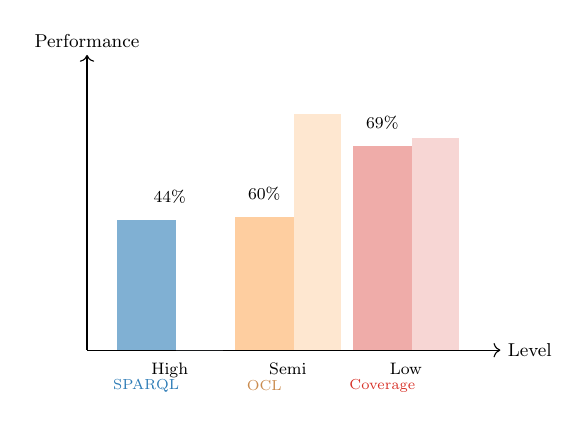
\begin{tikzpicture}[scale=0.75, transform shape]
\draw[->] (0,0) -- (7,0) node[right, font=\small] {Level};
\draw[->] (0,0) -- (0,5) node[above, font=\small] {Performance};

% Mistral bars
\fill[highformal!60] (0.5,0) rectangle (1.5,2.2);
\fill[semiformal!60] (2.5,0) rectangle (3.5,2.25);
\fill[lowformal!40] (4.5,0) rectangle (5.5,3.45);

% Llama bars (offset)
\fill[highformal!30] (1.5,0) rectangle (2.3,0);
\fill[semiformal!30] (3.5,0) rectangle (4.3,4.0);
\fill[lowformal!20] (5.5,0) rectangle (6.3,3.6);

% Labels
\node[font=\footnotesize, rotate=0] at (1.4,2.6) {44\%};
\node[font=\footnotesize] at (3.0,2.65) {60\%};
\node[font=\footnotesize] at (5.0,3.85) {69\%};

\node[font=\footnotesize, below] at (1.4,-0.1) {High};
\node[font=\footnotesize, below] at (3.4,-0.1) {Semi};
\node[font=\footnotesize, below] at (5.4,-0.1) {Low};

\node[font=\scriptsize, highformal] at (1.0,-0.6) {SPARQL};
\node[font=\scriptsize, semiformal!80!black] at (3.0,-0.6) {OCL};
\node[font=\scriptsize, lowformal] at (5.0,-0.6) {Coverage};
\end{tikzpicture}

\vspace{0.3em}
{\small\color{gray} Note: metrics differ per level --- direct comparison is illustrative, not statistical. Full experiment uses unified rubric.}
\end{column}
\end{columns}

\end{frame}

% ══════════════════════════════════════════════════════════════
\begin{frame}{Key Design Decisions}

\begin{enumerate}
    \item \textbf{Single domain eliminates the confound.}\\
    All three levels describe the same Northwind enterprise reality. The \emph{only} variable is formalization level.

    \vspace{0.5em}
    \item \textbf{CM artifacts at every level.}\\
    OWL 2 ontology / EER diagram / NL requirements --- representations Mylopoulos's framework was designed to classify.

    \vspace{0.5em}
    \item \textbf{Expert evaluation is non-negotiable.}\\
    Unified 0--3 rubric applied to all outputs by two annotators ($\kappa \geq 0.70$). No ``future work'' annotation.

    \vspace{0.5em}
    \item \textbf{EER uses structured prose, not PlantUML or JSON.}\\
    PlantUML is too code-like (collapses high--semi gap). JSON strips semantic conventions. Structured prose preserves the semi-formal character.

    \vspace{0.5em}
    \item \textbf{OCL fallback designed and ready.}\\
    If OCL fails at scale: constrained NL template preserves the formalization gradient.
\end{enumerate}

\end{frame}

% ══════════════════════════════════════════════════════════════
\begin{frame}{Contributions}

\begin{description}[C3:]
    \item[C1:] \textbf{Northwind CM Reasoning Benchmark}\\
    190 tasks spanning OWL/EER/NL over a single domain, with execution-verified and expert-annotated gold standards. Released under CC-BY.

    \vspace{0.5em}
    \item[C2:] \textbf{Automation Boundary in the CM Pipeline}\\
    Empirical identification of where LLM automation breaks down:\\
    {\small ``7--8B models achieve $X\%$ on SPARQL over OWL, $Y\%$ on OCL from EER, $Z\%$ entity coverage from NL --- domain held constant across all comparisons.''}

    \vspace{0.5em}
    \item[C3:] \textbf{SEQUAL-Grounded Formalization Metric}\\
    $F(T)$ as a measurement operationalization of SEQUAL syntactic, semantic, and pragmatic quality dimensions, with empirical LLM-performance correlates.
\end{description}

\end{frame}

% ══════════════════════════════════════════════════════════════
\begin{frame}{Implications for CM Tool Builders}

\begin{columns}[T]
\begin{column}{0.48\textwidth}
\textbf{Specific, actionable claims:}

\vspace{0.5em}
{\small
\begin{itemize}
    \item LLMs can reliably answer SPARQL competency questions over OWL 2 ontologies (accuracy $X\%$)
    \item LLMs cannot reliably synthesize OCL from EER annotations without verification ($Y\%$)
    \item Entity coverage from NL requirements is $Z\%$ --- the CIM-to-PIM step needs human support
\end{itemize}
}

\vspace{0.5em}
\textbf{Formalization ROI:}\\
{\small Moving from NL $\rightarrow$ EER yields $+Y$ points;\\EER $\rightarrow$ OWL yields $+Z$ further points.}
\end{column}

\begin{column}{0.48\textwidth}
\textbf{Variance paradox (from prior work):}

\vspace{0.5em}
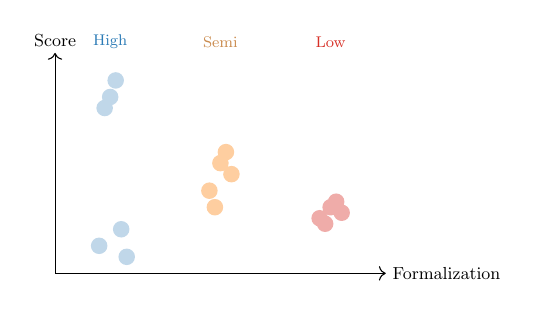
\begin{tikzpicture}[scale=0.7, transform shape]
\draw[->] (0,0) -- (6,0) node[right] {\small Formalization};
\draw[->] (0,0) -- (0,4) node[above] {\small Score};

% High-formal: bimodal
\fill[highformal!30] (0.8,0.5) circle (0.15);
\fill[highformal!30] (1.0,3.2) circle (0.15);
\fill[highformal!30] (1.2,0.8) circle (0.15);
\fill[highformal!30] (0.9,3.0) circle (0.15);
\fill[highformal!30] (1.1,3.5) circle (0.15);
\fill[highformal!30] (1.3,0.3) circle (0.15);

% Semi-formal: moderate spread
\fill[semiformal!60] (2.8,1.5) circle (0.15);
\fill[semiformal!60] (3.0,2.0) circle (0.15);
\fill[semiformal!60] (3.2,1.8) circle (0.15);
\fill[semiformal!60] (2.9,1.2) circle (0.15);
\fill[semiformal!60] (3.1,2.2) circle (0.15);

% Low-formal: tight cluster
\fill[lowformal!40] (4.8,1.0) circle (0.15);
\fill[lowformal!40] (5.0,1.2) circle (0.15);
\fill[lowformal!40] (5.2,1.1) circle (0.15);
\fill[lowformal!40] (4.9,0.9) circle (0.15);
\fill[lowformal!40] (5.1,1.3) circle (0.15);

\node[font=\footnotesize, highformal] at (1,4.2) {High};
\node[font=\footnotesize, semiformal!80!black] at (3,4.2) {Semi};
\node[font=\footnotesize, lowformal] at (5,4.2) {Low};
\end{tikzpicture}

\vspace{0.3em}
{\small Formal tasks: higher mean, higher variance\\(bimodal hit-or-miss)\\Informal tasks: lower mean, lower variance\\(consistently moderate)}
\end{column}
\end{columns}

\end{frame}

% ══════════════════════════════════════════════════════════════
\begin{frame}{Dual Publication Strategy}

\begin{table}
\centering
\small
\begin{tabular}{p{2cm}p{4.5cm}p{4.5cm}}
\toprule
& \textbf{ER 2026 (this paper)} & \textbf{NLP venue} \\
\midrule
Task types & OWL / EER / NL requirements & SQL / Legal clauses / Postmortems \\[0.3em]
Domain & Northwind (single domain) & Three different domains \\[0.3em]
Claim & Formalization gradient over CM artifacts & Cross-domain task-type generality \\[0.3em]
Theory & SEQUAL + Moody + Mylopoulos & Generic formalization hypothesis \\[0.3em]
Status & Pilot complete, scaling up & Results complete, paper drafted \\
\bottomrule
\end{tabular}
\end{table}

\vspace{0.5em}
\centering
Both papers share the statistical pipeline, $F(T)$ metric, and formalization hypothesis.\\
Neither is derivative of the other --- they establish the result in different contexts.

\end{frame}

% ══════════════════════════════════════════════════════════════
\begin{frame}{Timeline}

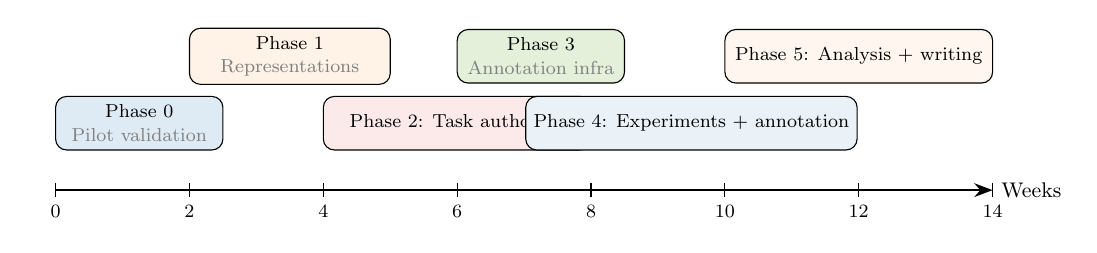
\begin{tikzpicture}[
    phase/.style={draw, rounded corners, minimum height=0.8cm, align=center, font=\small},
    scale=0.85, transform shape
]
% Timeline
\draw[-{Stealth}, thick] (0,0) -- (14,0) node[right] {\small Weeks};
\foreach \x in {0,2,4,6,8,10,12,14} {
    \draw (\x,0.1) -- (\x,-0.1) node[below, font=\footnotesize] {\x};
}

% Phases
\node[phase, fill=highformal!15, minimum width=2.5cm] at (1.25,1) {\footnotesize Phase 0\\[-0.1em]\footnotesize\color{gray}Pilot validation};
\node[phase, fill=semiformal!15, minimum width=3cm] at (3.5,2) {\footnotesize Phase 1\\[-0.1em]\footnotesize\color{gray}Representations};
\node[phase, fill=lowformal!10, minimum width=4cm] at (6,1) {\footnotesize Phase 2: Task authoring};
\node[phase, fill=nwgreen!15, minimum width=2.5cm] at (7.25,2) {\footnotesize Phase 3\\[-0.1em]\footnotesize\color{gray}Annotation infra};
\node[phase, fill=highformal!10, minimum width=4cm] at (9.5,1) {\footnotesize Phase 4: Experiments + annotation};
\node[phase, fill=semiformal!10, minimum width=4cm] at (12,2) {\footnotesize Phase 5: Analysis + writing};

% Checkmark for Phase 0
\node[font=\large, nwgreen] at (-0.3,1) {\checkmark};
\end{tikzpicture}

\vspace{1em}
\begin{itemize}\small
    \item Phase 0 (pilot): \textbf{Complete.} All pipeline components validated. Go/no-go decisions made.
    \item Phase 1--2 (representations + tasks): Full Northwind ontology, EER, NL + 190 tasks
    \item Phase 3--4 (annotation + execution): 1,900 records + expert scoring
    \item Phase 5--6 (analysis + submission): SEQUAL framing, automation-boundary claims
\end{itemize}

\end{frame}

% ══════════════════════════════════════════════════════════════
\begin{frame}{Summary}

\begin{enumerate}
    \item \textbf{Same domain, three formalizations.}\\
    Northwind represented as OWL 2 ontology, EER diagram, and NL requirements --- the CM representations Mylopoulos's framework classifies.

    \vspace{0.3em}
    \item \textbf{190-task benchmark with execution-verified and expert-annotated gold standards.}\\
    Independently valuable to the ER community.

    \vspace{0.3em}
    \item \textbf{Specific automation-boundary claims.}\\
    Where 7--8B LLMs can and cannot assist in the CM pipeline --- actionable for tool builders.

    \vspace{0.3em}
    \item \textbf{Pilot validates the pipeline.}\\
    HermiT, Jena, OCL parser, coverage script all tested. Both models produce interpretable outputs at all three levels. OCL go/no-go: proceed.
\end{enumerate}

\vspace{1em}
\centering
\textbf{The ER community's question:} Can LLMs reason over conceptual models?\\
\textbf{Our answer:} It depends --- measurably --- on the formalization level.

\end{frame}

\end{document}
